\begin{frame}[fragile]{\insertsubsection}
  \begin{columns}
    \begin{column}{0.5\textwidth}
      \begin{minted}[gobble = 4, frame = lines, framesep = 7pt, linenos,
        breaklines]{rust}
        enum Pohek {
          Xss(XssType),
          SocialEngineering,
          Phishing,
          // ...
        }

        enum XssType {
          Reflected,
          Stored,
          // ...
        }
      \end{minted}
    \end{column}
    \begin{column}{0.5\textwidth}
      \begin{minted}[gobble = 4, frame = lines, framesep = 7pt, linenos,
        breaklines]{rust}
        match pohek {
          Pohek::Xss(xss_type) =>
          {
            hack_by_xss(xss_type);
          },
          Pohek::SocialEngineering |
          Pohek::Phishing =>
          {
            pa3Becmu_JIOXA();
          }
          _ => {},
        }
      \end{minted}
    \end{column}
  \end{columns}

  \note {

    \textbf{Enum} в Rust используется для создания \textbf{алгебраических типов}
    --- можно создать один тип, который будет \textbf{включать себя сумму
      типов}. Да, во множестве языков есть алгебраические типы, но в Rust с ними
    также удобно работать, как и в других функциональных языках.

    Одним из ярких примеров удобства является \textbf{конструкция
      \texttt{match}}, заменяет \texttt{switch}, даёт гораздо больше
    возможностей, работает с деструктурированием данных, отслеживает полное
    покрытие всех типов, позволяет задавать условия и т. д.
  }
\end{frame}

\begin{frame}[fragile]{Option}
  \begin{minted}[gobble = 4, frame = lines, framesep = 7pt, linenos,
    breaklines]{rust}
    fn find_vulnerability(program: &Program) -> Option<Vulnerability> {...}

    fn hack_program(program: &mut Program) {
        match find_vulnerability(&program) {
            Some(vuln) => {
                exploit(vuln);
            }
            None => println!("Better luck next time."),
        }
    }
  \end{minted}

  \note {

    Когда мы пытаемся найти уязвимость, мы можем её либо найти, либо нет, так
    вот когда мы не находим уязвимость, нам ничего не возвращается, и мы об этом
    должны знать.

    Благодаря алгебраическим типам, \textbf{Rust обходится без Null}. Вместо
    него используется \textbf{алгебраический тип \texttt{Option}}, который может
    возвращать либо объект типа \textbf{\texttt{Some} с данными внутри}, либо
    объект \textbf{типа \texttt{None}}, который и является заменой Null.

    Всё это опять же пришло из функциональных языков.

  }
\end{frame}

\begin{frame}{Optional (C++)}

  \only<1>{%
    \begin{itemize}
    \item \texttt{std::optional}
    \item \texttt{std::variant}
    \item \texttt{std::any}
    \item \texttt{std::pair}
    \end{itemize}
  }%
  \only<2>{%
    \center%
    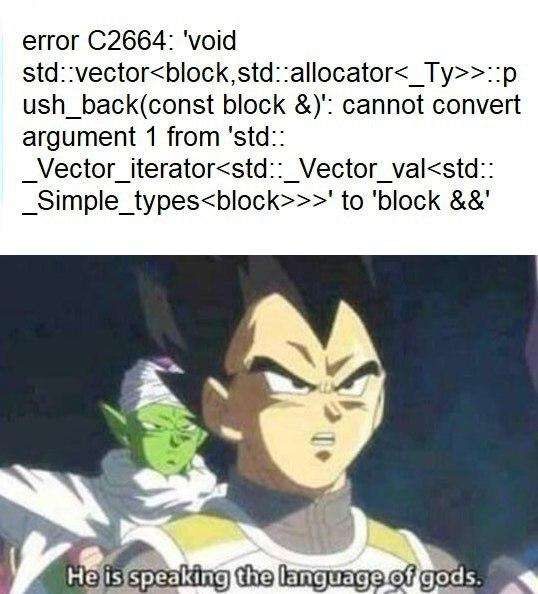
\includegraphics[height = 0.9\textheight]{gods_language.jpg}
  }%

  \note<1>{

    Кто разрабатывает на C++? Вы знали, что там есть подобные алгебраические
    типы?

    Если вы не знали, в C++ тоже есть подобные алгебраические типы, а также
    \texttt{std::optional} и \texttt{std::variant} с C++17, но там не всё так
    просто:

    \begin{itemize}
    \item иногда приходится проверять возвращаемый тип;
    \item приходится использовать либо boost, либо C++17, что вносит некоторую
      сумятицу;
    \item в случае ошибки же \textbf{выходит какой-то ад (next slide)}.
    \end{itemize}

  }

  \note<2>{

    Чего, кто, кого? Где ошибка?

    На самом деле так со всем в C++, где используются шаблоны или
    \textbf{параметризированные типы}.

  }

\end{frame}
